\mode*
\begin{frame}
  \frametitle{Aufbau des Verfahrens}
  \begin{figure}
    \centering
    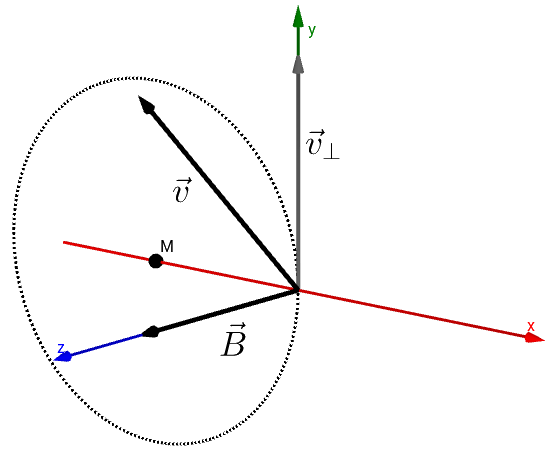
\includegraphics[width=0.6\textwidth]{../geogebra/img/local_movement_edited}
    \caption{Das lokale Koordinatensystem des im Ursprung befindlichen Ladungstr\"agers mit Andeutung der Kreisbahn in der
      \textit{xy}-Ebene.}
    \label{fig:locale_movement}
  \end{figure}
\end{frame}

\begin{frame}
  \frametitle{Aufbau des Verfahrens}
  \textbf{Die Flugbahn im lokalen Bezugssystem}
  \begin{itemize}
    \item \(v_\parallel\) verfolgt gleichf\"ormige Bewegung
    \item \(v_\perp\) verfolgt Kreisbewegung in der \textit{xy}-Ebene
    \item allgemeine Beschreibung von Kreisbewegungen in der Ebene:
  \end{itemize}
  \begin{equation*}
    \begin{pmatrix}
      x(t) \\
      y(t)
    \end{pmatrix}
    =
    \begin{pmatrix}
      r \cdot \sin{\left(\omega \cdot t\right)} + M_x \\
      r \cdot \cos{\left(\omega \cdot t\right)} + M_y
    \end{pmatrix}
  \end{equation*}
  \begin{itemize}
  \item unter Verwendung der bisherigen \"Uberlegungen ergibt sich konkret:
  \end{itemize}
  \begin{equation*}
    \begin{pmatrix}
      x(t) \\
      y(t) \\
      z(t)
    \end{pmatrix}
    =
    \begin{pmatrix}
      r \cdot \sin{\left(\omega \cdot t\right)} - r \\
      r \cdot \cos{\left(\omega \cdot t\right)} \\
      \vec{v}_z \cdot t
    \end{pmatrix}
  \end{equation*}
\end{frame}

\begin{frame}
  \frametitle{Aufbau des Verfahrens}
  \textbf{\"Ubertragung auf das globale Koordinatensystem}
  \begin{enumerate}
    \item Transformation von \(\vec{v}\) und \(\vec{B}\) in das lokale Bezugssystem des Teilchens (\(\rightarrow\) Basiswechsel)
    \item Anwendung der hergeleiteten Zusammenh\"ange im lokalen System \(\rightarrow\) neue Teilchenposition und Bewegungsrichtung
    \item R\"ucktransformation (\(\rightarrow\) Zur\"uck zur alten Basis)
  \end{enumerate}
  \begin{itemize}
    \item Hierzu: Verwendung von orthogonalen Transformationen
      \begin{itemize}
        \item Drehung von \(\vec{v}\) und \(\vec{B}\)
      \end{itemize}
    \item Eulersche Winkel
      \begin{itemize}
        \item erm\"oglichen Drehungen um bereits gedrehte Achsen
      \end{itemize}
    \item Wie lauten die Drehwinkel?
  \end{itemize}
\end{frame}

\begin{frame}
  \frametitle{Aufbau des Verfahrens}
  \begin{figure}
    \centering
    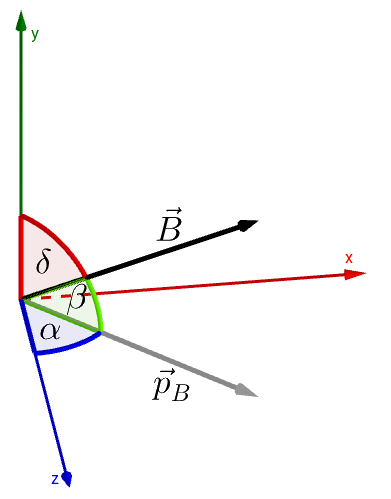
\includegraphics[width=0.4\textwidth]{../geogebra/img/winkel_edited}
    \caption{Illustration der Winkel \(\alpha\), \(\beta\) und \(\delta\), die zur Drehung der \(z\)-Achse ben\"otigt werden.}
    \label{fig:winkelfig}
  \end{figure}
\end{frame}

\begin{frame}
  \frametitle{Aufbau des Verfahrens}
  \begin{figure}
    \centering
    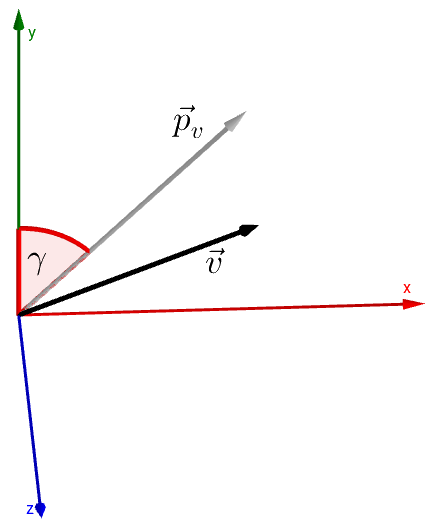
\includegraphics[width=0.4\textwidth]{../geogebra/img/winkel_v_edited}
    \caption{Darstellung des Winkels \(\gamma\), welcher zur Transformation von \(\vec{v}\) ben\"otigt wird.}
    \label{fig:winkelv}
  \end{figure}
\end{frame}

\begin{frame}
  \frametitle{Aufbau des Verfahrens}
  \textbf{Ausweitung auf inhomogene Magnetfelder}
  \begin{itemize}
    \item lokale Approximation durch ein homogenes Magnetfeld
      \begin{itemize}
        \item Diskretisierung des inhomogenen Feldes
      \end{itemize}
    \item Berechnung der neuen Position in der lokalen Approximation
    \item Generierung einer neuen Approximation nach jedem Update von Position und Bewegungsrichtung
      \begin{itemize}
        \item mehrere Iterationen
      \end{itemize}
    \item Zeit \(t\) als Diskretisierungsparameter
      \begin{itemize}
        \item wie "`lange"' soll das lokal homogene Modell verwendet werden?
      \end{itemize}
    \item je kleiner \(t\), desto genauer das Verfahren
    \item Wann endet die Simulation?
  \end{itemize}
\end{frame}

\begin{frame}
  \frametitle{Aufbau des Verfahrens}
  \textbf{Abbruchkriterien}
  \begin{itemize}
    \item Schnittpunkt der Flugbahn mit einer Ebene
      \begin{itemize}
        \item Bestimmte Bereiche im Detektor k\"onnen durch Ebenen abgetrennt werden
      \end{itemize}
    \item Zur\"ucklegen einer maximalen Distanz
      \begin{itemize}
        \item Verwendung eines Bezugspunktes zur Berechnung der Entfernung
      \end{itemize}
    \item Wechsel der Detektorgeometrie
      \begin{itemize}
        \item Stop der Iteration bei Eintritt in irrelevante Detektorabschnitte
      \end{itemize}
    \item Passieren eines bestimmten Ortes
      \begin{itemize}
        \item Stop der Iteration wenn Distanz zu gegebenem Ort minimal wird
      \end{itemize}
    \item logische Verkn\"upfungen der Bedingungen
    \item \ldots
  \end{itemize}
\end{frame}

\begin{frame}
  \frametitle{Aufbau des Verfahrens}
  \textbf{Der resultierende Algorithmus}\\
  \begin{itemize}
  \item solange Abbruchbedingung nicht erf\"ullt:
    \begin{enumerate}
    \item erfrage die Gr\"o{\ss}en \(\vec{B}\), \(\vec{v}\), sowie die aktuelle Position
    \item berechne die Winkel f\"ur die Basistransformation
    \item f\"uhre den Basiswechsel durch
    \item berechne die neue Position in der lokalen Basis und aktualisiere die Richtung von \(\vec{v}\)
    \item transformiere zur\"uck in die alte Basis
    \item speichere die neue Teilchenposition
    \end{enumerate}
  \end{itemize}
\end{frame}

\mode<all>
